
%Не забыть:
%--------------------------------------
%Вставить колонтитулы, поменять название на титульнике



%--------------------------------------

\documentclass[a4paper, 12pt]{article} 

%--------------------------------------
%Russian-specific packages
%--------------------------------------
%\usepackage[warn]{mathtext}
\usepackage[T2A]{fontenc}
\usepackage[utf8]{inputenc}
\usepackage[english,russian]{babel}
\usepackage[intlimits]{amsmath}
\usepackage{esint}
%--------------------------------------
%Hyphenation rules
%--------------------------------------
\usepackage{hyphenat}
\hyphenation{ма-те-ма-ти-ка вос-ста-нав-ли-вать}
%--------------------------------------
%Packages
%--------------------------------------
\usepackage{amsmath}
\usepackage{amssymb}
\usepackage{amsfonts}
\usepackage{amsthm}
\usepackage{latexsym}
\usepackage{mathtools}
\usepackage{epstopdf}
\usepackage{etoolbox}%Булевые операторы
\usepackage{extsizes}%Выставление произвольного шрифта в \documentclass
\usepackage{geometry}%Разметка листа
\usepackage{indentfirst}
\usepackage{wrapfig}%Создание обтекаемых текстом объектов
\usepackage{fancyhdr}%Создание колонтитулов
\usepackage{setspace}%Настройка интерлиньяжа
\usepackage{lastpage}%Вывод номера последней страницы в документе, \lastpage
\usepackage{soul}%Изменение параметров начертания
\usepackage{hyperref}%Две строчки с настройкой гиперссылок внутри получаеммого
\usepackage[usenames,dvipsnames,svgnames,table,rgb]{xcolor}% pdf-документа
\usepackage{multicol}%Позволяет писать текст в несколько колонок
\usepackage{cite}%Работа с библиографией
\usepackage{subfigure}% Человеческая вставка нескольких картинок
\usepackage{tikz}%Рисование рисунков
\usepackage{float}
% Для картинок Моти
\usepackage{misccorr}
\usepackage{lscape}
\usepackage{cmap}


\usepackage{graphicx,xcolor}
\graphicspath{{Pictures/}}
\DeclareGraphicsExtensions{.pdf,.png,.jpg}

%----------------------------------------
%Список окружений
%----------------------------------------
\newenvironment {theor}[2]
{\smallskip \par \textbf{#1.} \textit{#2}  \par $\blacktriangleleft$}
{\flushright{$\blacktriangleright$} \medskip \par} %лемма/теорема с доказательством
\newenvironment {proofn}
{\par $\blacktriangleleft$}
{$\blacktriangleright$ \par} %доказательство
%----------------------------------------
%Список команд
%----------------------------------------



\newcommand{\grad}
{\mathop{\mathrm{grad}}\nolimits} %градиент

\newcommand{\diver}
{\mathop{\mathrm{div}}\nolimits} %дивергенция

\newcommand{\Def}[1]
{\underline{\textbf{#1}}} %определение

\newcommand{\RN}[1]
{\MakeUppercase{\romannumeral #1}} %римские цифры

\newcommand {\theornp}[2]
{\textbf{#1.} \textit{ #2} \par} %Написание леммы/теоремы без доказательства

\newcommand{\qrq}
{\ensuremath{\quad \Rightarrow \quad}} %Человеческий знак следствия

\newcommand{\qlrq}
{\ensuremath{\quad \Leftrightarrow \quad}} %Человеческий знак равносильности

\renewcommand{\phi}{\varphi} %Нормальный знак фи

\newcommand{\me}
{\ensuremath{\mathbb{E}}}

\newcommand{\md}
{\ensuremath{\mathbb{D}}}



%\renewcommand{\vec}{\overline}




%----------------------------------------
%Разметка листа
%----------------------------------------
\geometry{top = 3cm}
\geometry{bottom = 2cm}
\geometry{left = 0.7cm}
\geometry{right = 0.7cm}
%----------------------------------------
%Колонтитулы
%----------------------------------------
\pagestyle{fancy}%Создание колонтитулов
\fancyhead{}
%\fancyfoot{}
\fancyhead[C]{\textsc{Дифракция Фраунгофера на решётке}}%Вставить колонтитул сюда
%----------------------------------------
%Интерлиньяж (расстояния между строчками)
%----------------------------------------
%\onehalfspacing -- интерлиньяж 1.5
%\doublespacing -- интерлиньяж 2
%----------------------------------------
%Настройка гиперссылок
%----------------------------------------
\hypersetup{				% Гиперссылки
	unicode=true,           % русские буквы в раздела PDF
	pdftitle={Заголовок},   % Заголовок
	pdfauthor={Автор},      % Автор
	pdfsubject={Тема},      % Тема
	pdfcreator={Создатель}, % Создатель
	pdfproducer={Производитель}, % Производитель
	pdfkeywords={keyword1} {key2} {key3}, % Ключевые слова
	colorlinks=true,       	% false: ссылки в рамках; true: цветные ссылки
	linkcolor=blue,          % внутренние ссылки
	citecolor=blue,        % на библиографию
	filecolor=magenta,      % на файлы
	urlcolor=cyan           % на URL
}
%----------------------------------------
%Работа с библиографией (как бич)
%----------------------------------------
\renewcommand{\refname}{Список литературы}%Изменение названия списка литературы для article
%\renewcommand{\bibname}{Список литературы}%Изменение названия списка литературы для book и report
%----------------------------------------
\begin{document}
\begin{titlepage}
\begin{center}
\textsc{Национальный исследовательский университет "Высшая школа экономики"\\[5mm]
Факультет Физики}

\vfill

\textbf{ОТЧЁТ ПО ЛАБОРАТОРНОЙ РАБОТЕ \\[3mm]
"ДИФРАКЦИЯ ФРАУНГОФЕРА НА РЕШЁТКЕ"\\[3mm]
по курсу "Оптика"
\\[20mm]
}
\end{center}

\hfill
\begin{minipage}{.5\textwidth}
Выполнила:\\[2mm] 
Фазлиахметова Олеся Камилевна\\
БФЗ193\\
2 курс\\[5mm]

Проверила:\\[2mm] 
Готовко С. К. 
\end{minipage}%
\vfill
\begin{center}
 Москва\\
 \today
\end{center}
\end{titlepage}



\tableofcontents

\newpage

	\section{Цель работы}

Перед началом выполнения работы были поставлены следующие цели:

\begin{enumerate}

	\item Собрать установку для наблюдения дифракции на отражающей дифракционно решетке, изучить дифракционную картику для различных решёток при различных углах падения света на решетку $\Theta_i$, определить положения максимумов.

	\item Для каждой решетки определить число штрихов на единицу длины d.

	\item С помощью фотодиодного измерителя мощности измерить интенсивность света в максимумах для решетки, с помощью которой наблюдается наибольшее количество максимумов. Обработав получнную зависимость, определить угол скоса решётки $\gamma$.

\end{enumerate}

\section{Оборудование}

\begin{enumerate}

	\item Лазеры с длиной волны $\lambda = 520 $ нм;

	\item Отражающие дифракционные решетки с разными постоянными решетки;

	\item Переносной экран;

	\item Подставки и крепления для элементов оптической схемы;

	\item Линейки.

\end{enumerate}

\section{Теоретическое описание}


\subsection{Дифракционная решетка}

Дифракционная решётка представляет собой периодическую структуру одинаковых щелей с периодом $d$. Пусть плоская монороматическая волна (с длиной волны $\lambda$) падает на решетку перпендикулярно к ее поверхности. Здесь также точка  наблюдения P находится под углом $\Theta$ (угол дифракции) к нормали к решетке. Тогда результирующее поле в точке Р, излучаемое всеми N щелями:
\begin{equation}
E(\Theta) = E_1(\Theta)e^{i\delta(N/2-1)}\frac{\sin(N\delta/2)} {\sin(\delta/2)},\;\;\;\; \delta = kd\sin(\Theta)
\end{equation}
\[ E_1(\Theta) \propto \frac{\sin(kb/2\sin\Theta)} {(kb/2\sin\Theta}, \;\;\;\; b\text{ -- ширина щели}\]

Распределение интенсивности по углам описывается следующим соотношением:

\begin{equation}
I \propto \left[\frac{\sin(kb/2(\sin\Theta+\sin\Theta_i))} {(kb/2(\sin\Theta+\sin\Theta_i)} \frac{\sin(Nkd/2(\sin\Theta+\sin\Theta_i))} {\sin(kd/2(\sin\Theta+\sin\Theta_i))}\right]^2
\end{equation}

Положения максимумов определяются из условия:

\begin{equation}
d(\sin\Theta+\sin\Theta_i) = m\lambda, \;\;\;\; m\in\mathrm{Z} \text{ -- порядок максимума.}
\end{equation}


\begin{figure}[H]
	\centering
	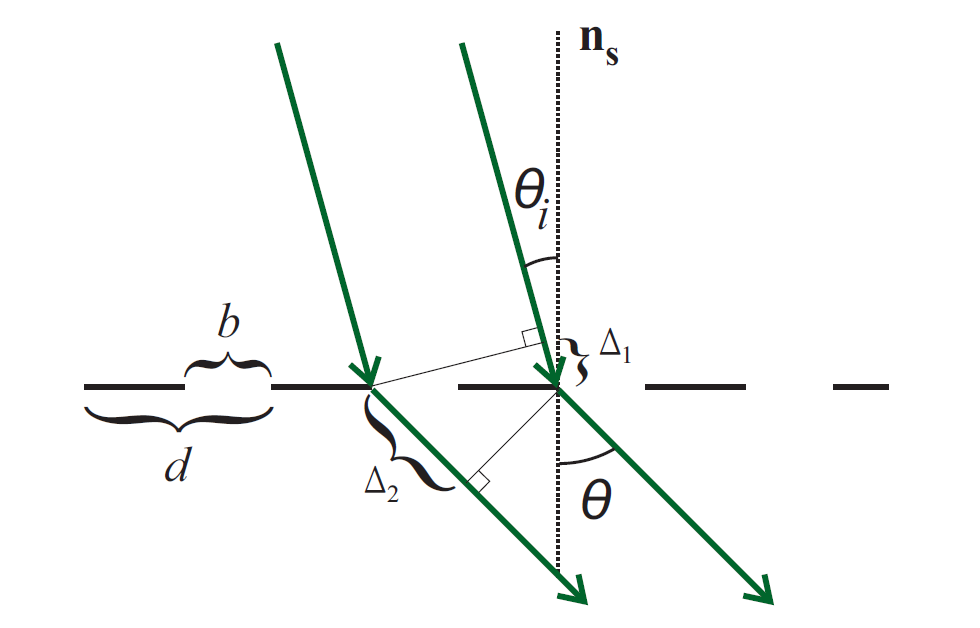
\includegraphics[scale=0.6]{1}
	\caption{Дифракция Фраунгофера на решетке}
\end{figure}


\subsection{Концентрирующая отражающая решетка (blazed grating)}

Для практических целей часто используются отражающие решетки с треугольным профилем. Такие решетки позволяют концентрировать дифрагировавшее излучение в ненулевом порядке. Такая решетка характеризуется углом скоса ($\gamma$), определяющием, в каком порядке $m$ будет наблюдаться максимум дифрагировавшего излучения в зависимотси от длины волны (см. Рис. 2). 

\begin{figure}[H]
	\centering
	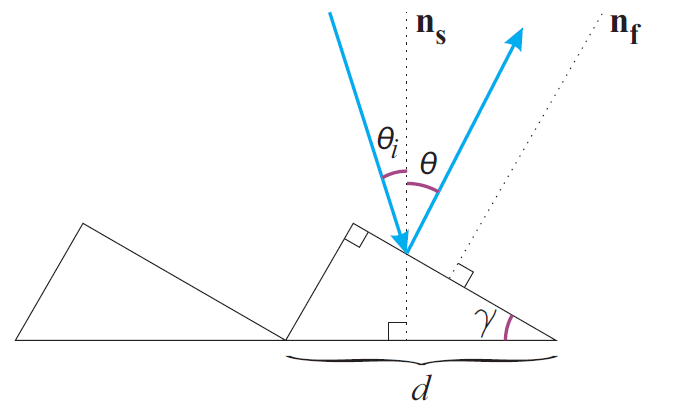
\includegraphics[scale=0.6]{2}
	\caption{Концентрирующая отражающая решетка (blazed grating)}
\end{figure}


Распределение интенсивности (2) преобразуется следующим образом:

\begin{equation}
I \propto \left[\frac{\sin(kd\cos\gamma/2(\sin(\Theta-\gamma)+\sin(\Theta_i-\gamma)))} {kd\cos\gamma/2(\sin(\Theta-\gamma)+\sin(\Theta_i-\gamma))} \frac{\sin(Nkd/2(\sin\Theta+\sin\Theta_i))} {\sin(kd/2(\sin\Theta+\sin\Theta_i))}\right]^2
\end{equation}

\section{Выполнение работы}

\subsection{Определение положения максимумов при различных углах $\Theta_i$}
Погрешность измерения рулетки: $\pm0.1$ см. Примем за погрешность радиус пятна главного максимума $\pm0.2$.
\subsubsection{Решетка №1}
Положение нуля $l = 100$ см, расстрояние от решетки до стены $h = 119.5$ см.



$1. \; \Theta_i = 0$\\
\begin{center}
\begin{tabular}{| c| c | c |}
\hline
m  &  Расстояние, см & $\sin\Theta $\\ 
\hline
0. &  100. $\pm0.2$ & 0.\\
1. &  138.7$\pm0.2$  & 0.31\\
2. &  195. $\pm0.2$ & 0.62\\
-1.  & 61.2$\pm0.2$  &  -0.31\\
-2. & 6.9 $\pm0.2$ &  -0.61\\
\hline
\end{tabular}
\end{center}


$2. \; \Theta_i = 0.26$\\
\begin{center}
\begin{tabular}{| c| c | c |}
\hline
m  &  Расстояние, см & $\sin\Theta $\\ 
\hline
1.000e+00 & 1.100e+02$\pm0.2$  & 8.000e-02\\
2.000e+00 & 1.512e+02$\pm0.2$  & 3.900e-01\\
3.000e+00 & 2.190e+02$\pm0.2$   &7.100e-01\\
0.000e+00 & 7.230e+01$\pm0.2$  &-2.300e-01\\
-1.000e+00 & 2.480e+01 $\pm0.2$ & -5.300e-01\\
\hline
\end{tabular}
\end{center}




\subsubsection{Решетка №2}'


Положение нуля $l = 143.8$ см, расстрояние от решетки до стены $h = 119.5$ см.



$1. \; \Theta_i = 0$\\
\begin{center}
\begin{tabular}{| c| c | c |}
\hline
m  &  Расстояние, см & $\sin\Theta $\\ 
\hline
0. &  143.8$\pm0.2$    & 0. \\
1. &  239.  $\pm0.2$ &  0.62\\
-1.  & 49.  $\pm0.2$ & -0.62\\
\hline
\end{tabular}
\end{center}


$2. \; \Theta_i = 0.685$\\
\begin{center}
\begin{tabular}{| c| c | c |}
\hline
m  &  Расстояние, см & $\sin\Theta $\\ 
\hline
1. &  143.8 $\pm0.2$  &  0. \\
0.  &  48.5 $\pm0.2$ &  -0.62\\
\hline
\end{tabular}
\end{center}


\subsubsection{Решетка №3}
Положение нуля $l = 188.5$ см, расстрояние от решетки до стены $h = 122$ см.


$1. \; \Theta_i = 0$\\
\begin{center}
\begin{tabular}{| c| c | c |}
\hline
m  &  Расстояние, см & $\sin\Theta $\\ 
\hline
-5.000e+00 & 3.620e+01 $\pm0.2$ & -7.800e-01\\
 -4.000e+00 & 9.050e+01$\pm0.2$  & -6.300e-01\\
 -3.000e+00 & 1.235e+02$\pm0.2$  & -4.700e-01\\
 -2.000e+00 & 1.483e+02$\pm0.2$  & -3.100e-01\\
 -1.000e+00 & 1.693e+02$\pm0.2$  & -1.600e-01\\
  0.000e+00 & 1.885e+02$\pm0.2$  & 0.000e+00\\
  1.000e+00 & 2.073e+02$\pm0.2$  & 1.500e-01\\
  2.000e+00 & 2.280e+02$\pm0.2$  & 3.100e-01\\
  3.000e+00 & 2.525e+02$\pm0.2$  & 4.600e-01\\
  4.000e+00 & 2.851e+02$\pm0.2$  & 6.200e-01\\
  5.000e+00 & 3.395e+02$\pm0.2$  & 7.800e-01\\
\hline
\end{tabular}
\end{center}



$2.\; \Theta_i = 0.152$\\
\begin{center}
\begin{tabular}{| c| c | c |}
\hline
m  &  Расстояние, см & $\sin\Theta $\\ 
\hline
 1.000e+00 & 1.885e+02 $\pm0.2$ & 0.000e+00\\
 2.000e+00 & 2.287e+02 $\pm0.2$ & 3.100e-01\\
 3.000e+00 & 2.533e+02 $\pm0.2$ & 4.700e-01\\
 4.000e+00 & 2.860e+02 $\pm0.2$ & 6.200e-01\\
 5.000e+00 & 3.405e+02 $\pm0.2$ & 7.800e-01\\
 0.000e+00 & 1.695e+02$\pm0.2$  & -1.500e-01\\
-1.000e+00 & 1.243e+02$\pm0.2$  & -4.700e-01\\
-2.000e+00 & 9.130e+01 $\pm0.2$ & -6.200e-01\\
-3.000e+00 & 3.750e+01$\pm0.2$  & -7.800e-01\\
\hline
\end{tabular}
\end{center}





$3. \;\Theta_i = 0.29$\\
\begin{center}
\begin{tabular}{| c| c | c |}
\hline
m  &  Расстояние, см & $\sin\Theta $\\ 
\hline
 1.000e+00 & 1.710e+02$\pm0.2$  & -1.400e-01 \\
 2.000e+00 & 1.900e+02$\pm0.2$  & 1.000e-02 \\
 3.000e+00 & 2.098e+02$\pm0.2$  & 1.700e-01  \\
 4.000e+00 & 2.555e+02$\pm0.2$  & 4.800e-01  \\
 5.000e+00 & 2.900e+02$\pm0.2$  & 6.400e-01  \\
 0.000e+00 & 1.507e+02$\pm0.2$  & -3.000e-01  \\
-1.000e+00 & 1.267e+02$\pm0.2$  & -4.500e-01  \\
-2.000e+00 & 9.520e+01$\pm0.2$  & -6.100e-01 \\
\hline
\end{tabular}
\end{center}


$4.\; \Theta_i = 0.3855$\\
\begin{center}
\begin{tabular}{| c| c | c |}
\hline
m  &  Расстояние, см & $\sin\Theta $\\ 
\hline
 1.000e+00 & 1.642e+02$\pm0.2$  &-2.000e-01 \\
 2.000e+00 & 1.837e+02$\pm0.2$  &-4.000e-02 \\
 3.000e+00 & 2.230e+02$\pm0.2$  & 2.700e-01 \\
 4.000e+00 & 2.763e+02$\pm0.2$  & 5.800e-01 \\
 5.000e+00 & 3.230e+02$\pm0.2$  & 7.400e-01 \\
 0.000e+00 & 1.427e+02$\pm0.2$  &-3.500e-01 \\
-1.000e+00 & 1.167e+02$\pm0.2$  &-5.100e-01 \\
-2.000e+00 & 8.050e+01$\pm0.2$  &-6.600e-01 \\
-3.000e+00 & 1.550e+01$\pm0.2$  &-8.200e-01 \\
\hline
\end{tabular}
\end{center}






\subsection{Определение числа штрихов на единицу длины $a$}

Для каждой решетки построим зависимость $\sin\Theta(m)$. Она линейна -- коэффициент наклона прямой определяет величину $\lambda/d$.

\subsubsection{Решетка №1}
Число штрихов на единицу длины $a =595.5 \pm 0.5 \text{ мм}^{-1}$.

\begin{figure}[H]
	\centering
	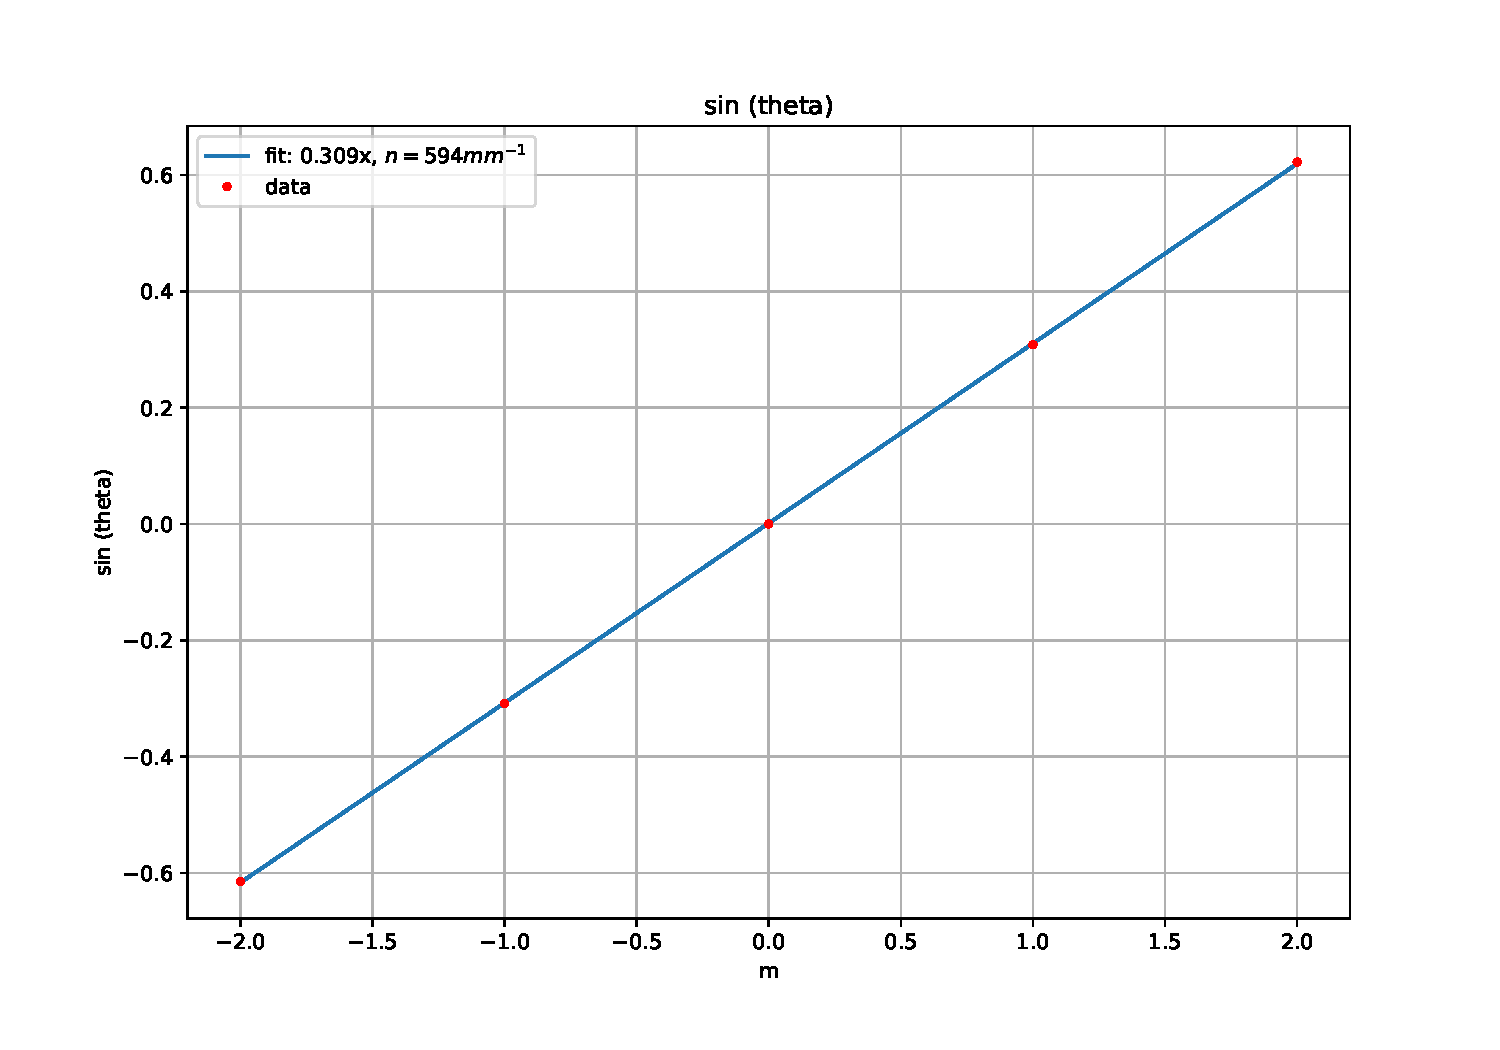
\includegraphics[scale=0.5]{1_0}
	\caption{$\Theta_i = 0$}
\end{figure}

\begin{figure}[H]
	\centering
	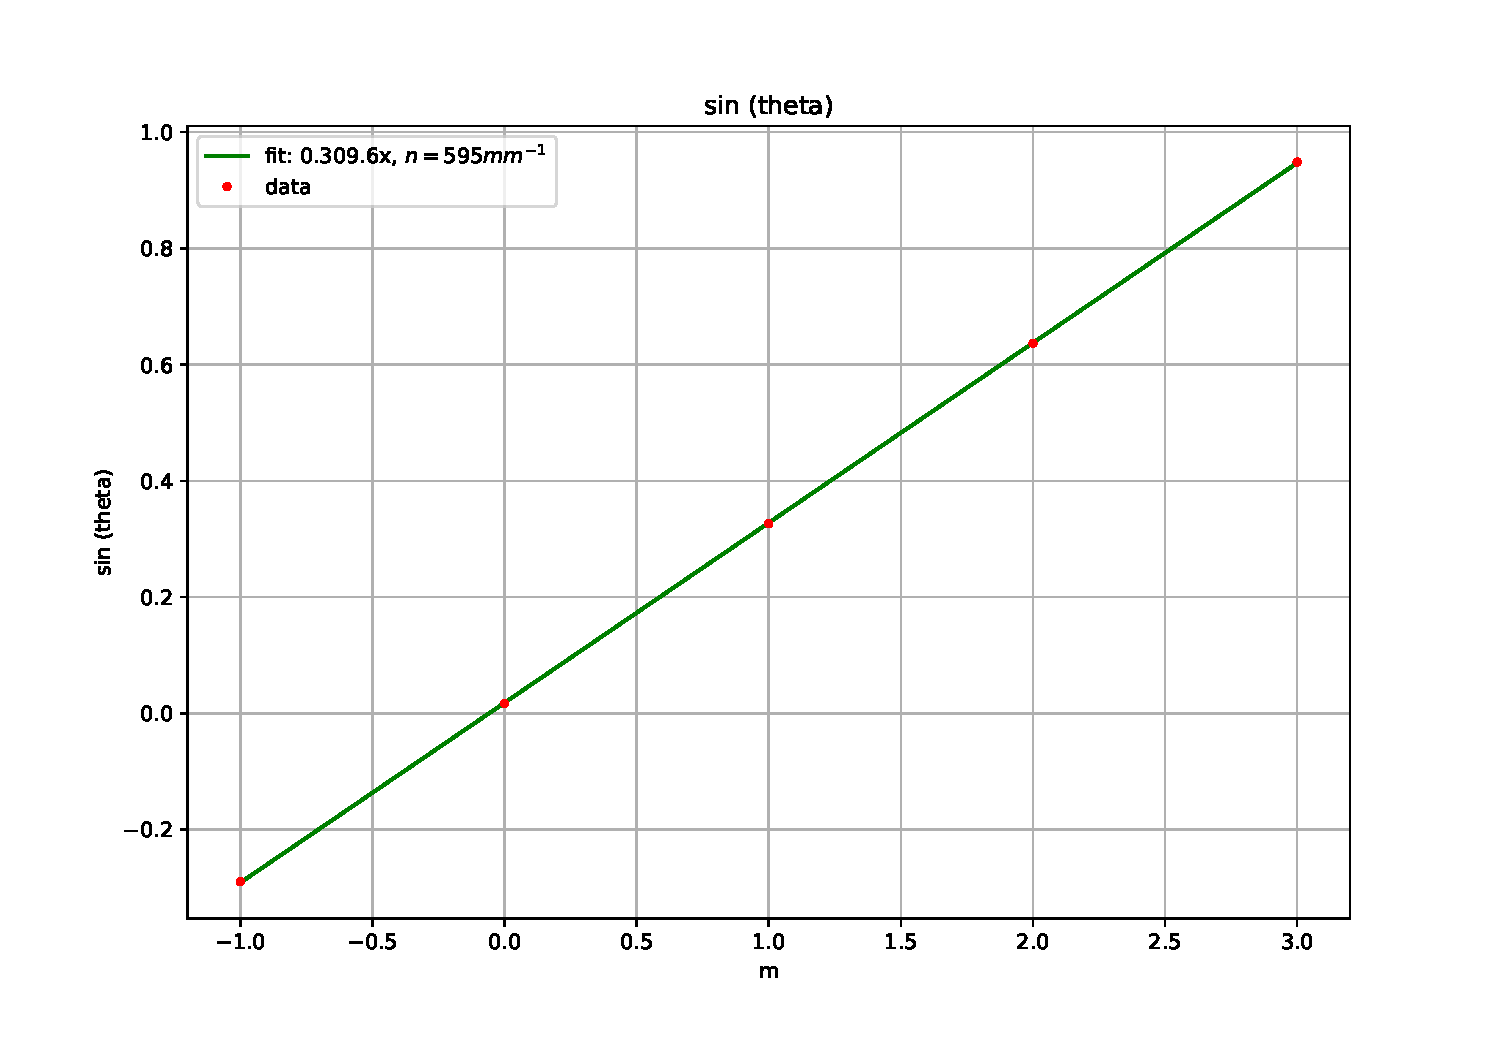
\includegraphics[scale=0.5]{1_2}
	\caption{$ \Theta_i = 0.26$}
\end{figure}



\subsubsection{Решетка №2}
Число штрихов на единицу длины $a = 1198 \pm 1  \text{ мм}^{-1}$.

\begin{figure}[H]
	\centering
	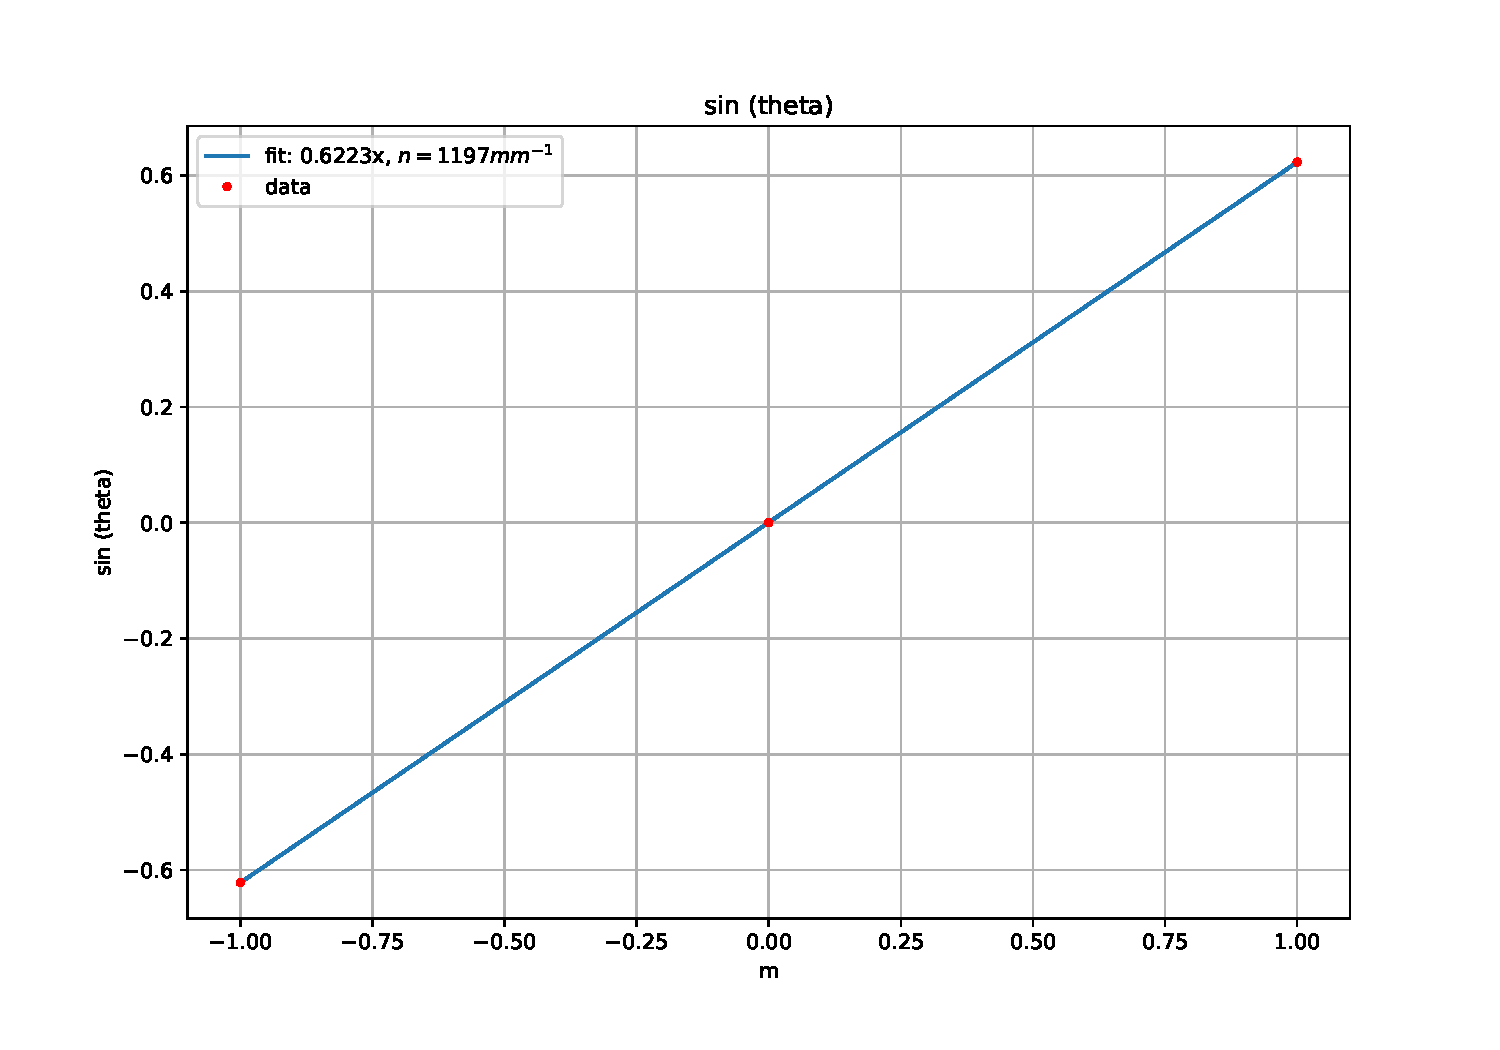
\includegraphics[scale=0.55]{2_0}
	\caption{$ \Theta_i = 0$}
\end{figure}


\begin{figure}[H]
	\centering
	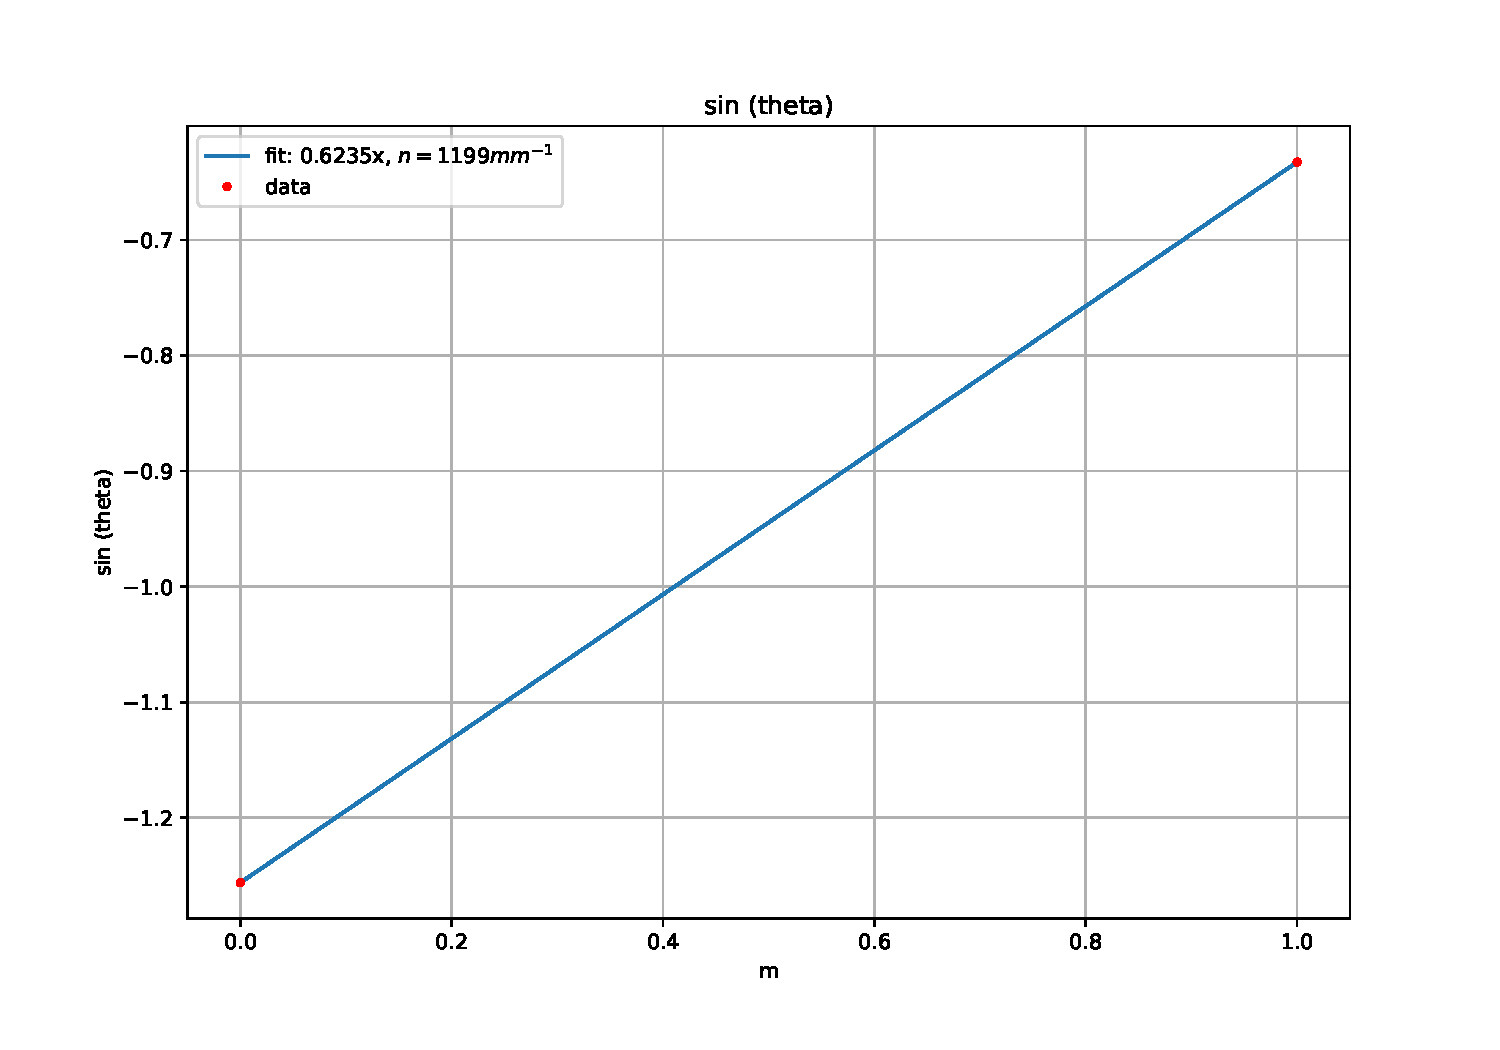
\includegraphics[scale=0.55]{2_1}
	\caption{$ \Theta_i = 0.685$}
\end{figure}




\subsubsection{Решетка №3}
Число штрихов на единицу длины $a = 325 \pm 25 \text{ мм}^{-1}$.

\begin{figure}[H]
	\centering
	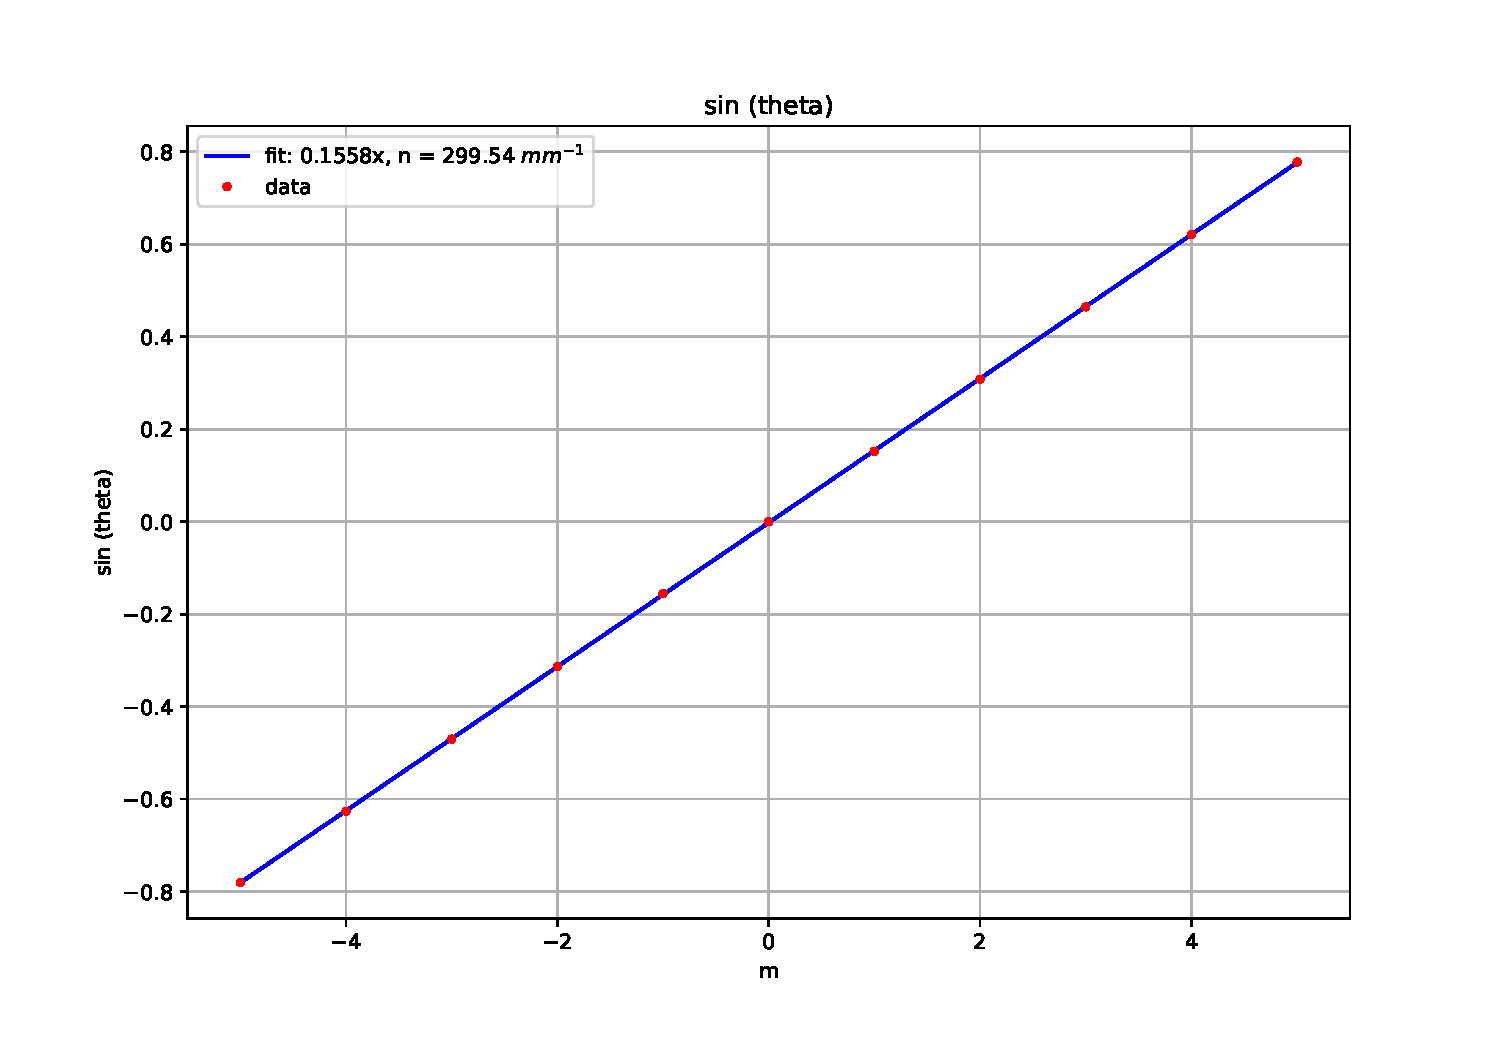
\includegraphics[scale=0.55]{3_0}
	\caption{$ \Theta_i = 0$}
\end{figure}

\begin{figure}[H]
	\centering
	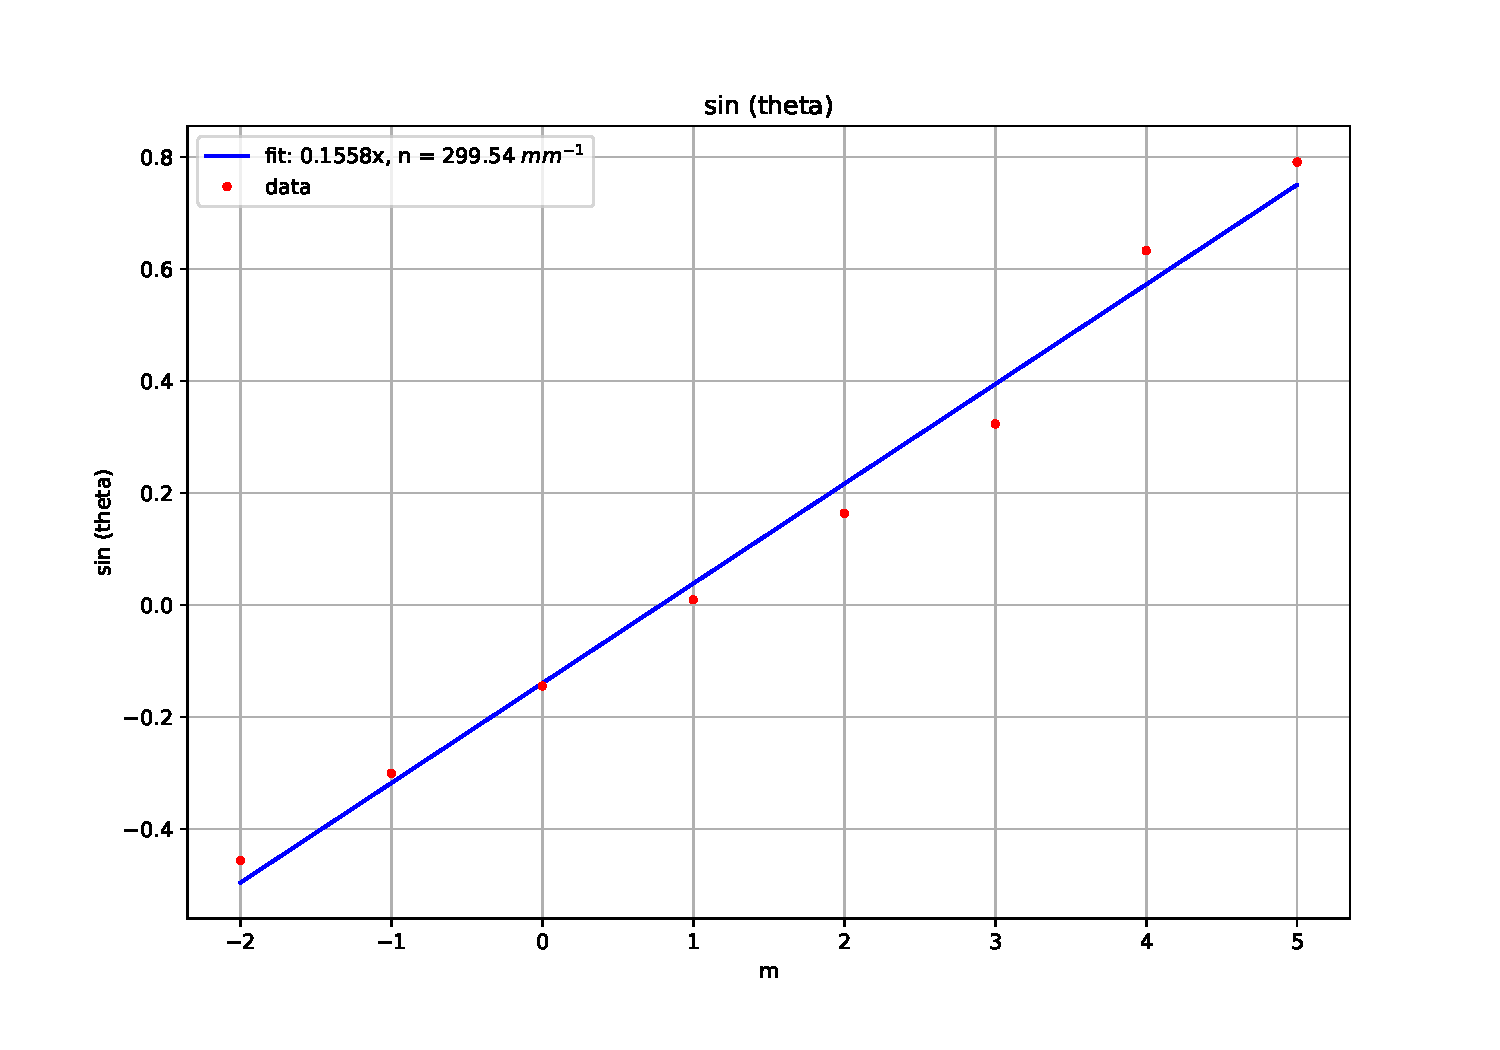
\includegraphics[scale=0.55]{3_2}
	\caption{$\Theta_i = 0.29$}
\end{figure}


\begin{figure}[H]
	\centering
	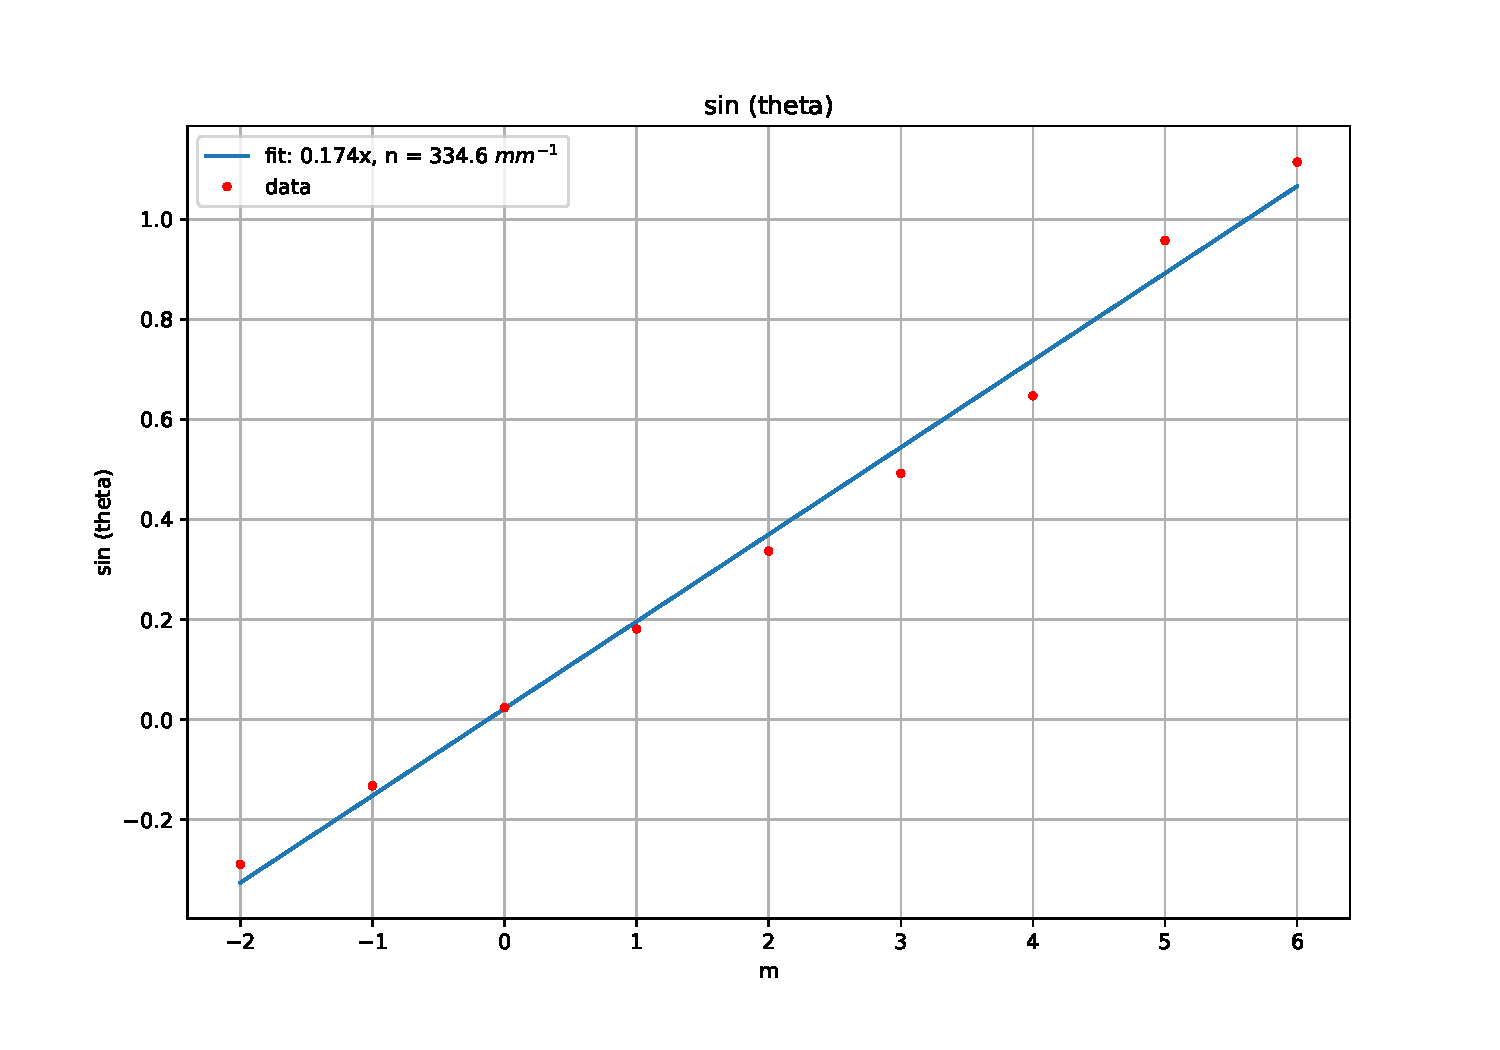
\includegraphics[scale=0.6]{3_4}
	\caption{$1\Theta_i = 0.45$}
\end{figure}





\subsection{Определение угла скоса решетки $\gamma$.}

Данные, которые были замерены с помощью фотодиодного измерителя мощности для решетки №3:


\begin{center}
\begin{tabular}{| c| c |}
\hline
Интенсивность, мВт  &  $\sin\Theta$\\ 
\hline
7.70e+01 & -7.80e-01\\
 8.00e+01 & -6.30e-01\\
 8.40e+01 & -4.70e-01\\
 1.00e+02 & -3.10e-01\\
 1.49e+02 & -1.60e-01\\
 4.94e+02 & 0.00e+00\\
 7.36e+03 & 1.50e-01\\
 7.60e+01 & 3.10e-01\\
 1.30e+01 & 4.60e-01\\
 1.60e+01 & 6.20e-01\\
1.50e+01 & 7.80e-01\\
\hline
\end{tabular}
\end{center}

Для нахождения угла скоса $\gamma$ аппроксимируем эти результаты функцией (4) и найдем ее параметры(указаны на Рис. 10):

\begin{figure}[H]
	\centering
	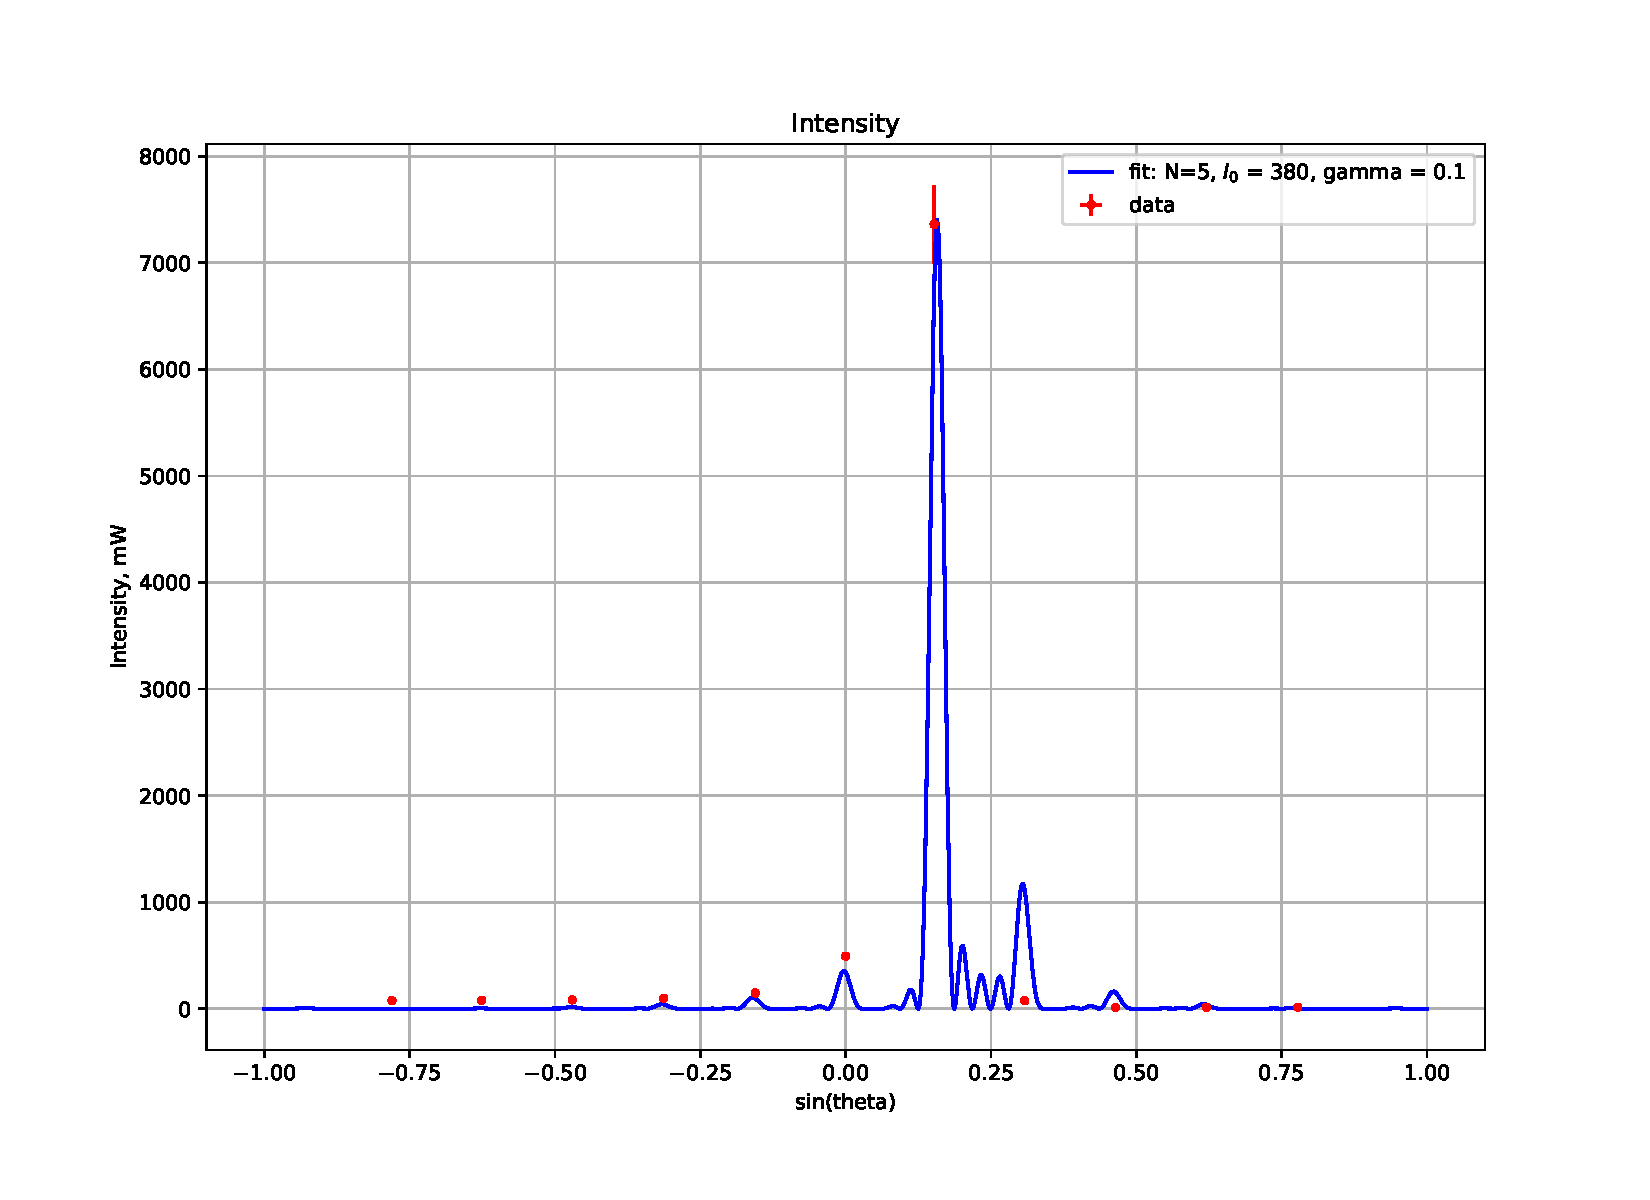
\includegraphics[scale=0.65]{Intensity.pdf}
	\caption{Интенсивность излучения}
\end{figure}
Погрешность измерения мощности лазерного излучения фотодиодным измерителем не превышает 5\%.

Т. о. угол скоса $\gamma = 0.1 \approx \frac {\pi}{30}$.

\subsection{Подсчет погрешностей}



\section{Вывод}

В ходе работы мы
 \begin{itemize}

	\item собрали установку для наблюдения дифракции на отражающей дифракционно решетке, изучили дифракционную картику для различных решёток при различных углах падения света на решетку $\Theta_i$, определили положения максимумов,

	\item для каждой решетки определили число штрихов на единицу длины $а$, эти значения оказались равными: 
		 \begin{enumerate}
			\item $a_1 = 595.5 \pm 0.5 $ мм
			\item $a_2 = 1198 \pm 1 $ мм
			\item $a_3 = 325 \pm 25 $ мм
		 \end{enumerate}

	\item с помощью фотодиодного измерителя мощности измерили интенсивность света в максимумах для решетки, с помощью которой наблюдается наибольшее количество максимумов. Обработав получнную зависимость, определили угол скоса решётки $\gamma$. Он оказался равен $\gamma = 0.1 \approx \frac {\pi}{30}$.

\end{itemize}
\end{document}